\section{Linguaggi ed espressioni regolari}
I \emph{linguaggi regolari} sono la famiglia più semplice di linguaggi formali, questo perché possono essere definiti in diversi modi:
\begin{itemize}
	\item Algebricamente.
	\item Attraverso grammatiche generative.
	\item Attraverso algoritmi di riconoscimento (\emph{automi})
\end{itemize}
Le \emph{espressioni regolari} (\emph{regexp}) sono stringhe \emph{r} definite attraverso i caratteri di un alfabeto $ \Sigma $ e mediante l'utilizzo dei meta-simboli $ \varnothing, \cup, \cdot, \ast $ attraverso l'applicazione e la combinazione delle seguenti regole
\begin{itemize}
	\item $ r= \varnothing $
	\item $ r = a, a\in \Sigma $
	\item $ r = (s \cup t) $
	\item $ r = (s\cdot t) \ o \ r = (st) $
	\item $ r = (s)^\ast $
\end{itemize}
Oltre a questi simboli talvolta, per semplificare la notazione, si utilizzano anche i simboli $ \varepsilon = \varnothing^\ast$ e $ r^+ = e\cdot e^\ast $.\\
Il risultato di un'espressione regolare \emph{e} è un linguaggio $ L_e $ costruito sull'alfabeto $ \Sigma $ che rispecchia le regole di \tablename\ref{tab:reggen}
\begin{table}
	\centering
\begin{tabular}{|c|c|}
	\hline \textbf{regexp} & \textbf{Linguaggio} \\ 
	\hline $ \varepsilon $ & $ \{\varepsilon\} $ \\ 
	\hline $ a\in\Sigma $ & $ \{a\} $ \\ 
	\hline $ s\cup t $ & $ L_s \cup L_t $ \\ 
	\hline $ s\cdot t $ & $ L_s\cdot L_t $ \\ 
	\hline $ s^\ast $ & $ L_s^\ast $ \\ 
	\hline 
\end{tabular}
\caption{Regole di generazione dei linguaggi da regexp}\label{tab:reggen}
\end{table}
A questo punto possiamo dire che un linguaggio è \emph{regolare} se è generato tramite l'utilizzo di \emph{espressioni regolari} come ad esempio
$$ e = (111)^* \quad L_e=\{1^{3n}|n = 0,1,\dots \} $$
\subsection{La famiglia dei linguaggi regolari}
Definiamo la \emph{famiglia dei linguaggi regolari} (\texttt{REG}) come la collezione di tutti i linguaggi regolari, inoltre, definiamo la \emph{famiglia dei linguaggi finiti} (\texttt{FIN}) la collezione di tutti i linguaggi aventi \emph{cardinalità finita}.\\
Ogni linguaggio finito è regolare in quanto è l'unione ($ \cup $) di un numero finito di stringhe le quali sono il concatenamento ($ \cdot $) di un numero finito di caratteri. Tuttavia l'insieme dei linguaggi regolari contiene anche linguaggi non finiti perciò l'inclusione risulta essere stretta.
$$FIN\subset REG$$
\subsection{Sottoespressione di un'espressione regolare}
Consideriamo un espressione completamente parentesizzata come la seguente:
$$e = (a \cup (bb))^\ast(c^+\cup(a \cup (bb)))$$
A questo punto distinguiamo tutti i termini numerandoli
$$e = (a_1 \cup (b_2b_3))^\ast(c_4^+\cup(a_5 \cup (b_6b_7)))$$
Infine mettiamo in evidenza tutte le sotto espressioni come mostrato in \figurename\ref{fig:scompo}
\begin{figure}
	\centering
	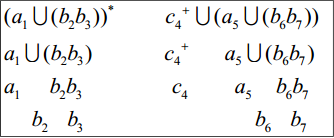
\includegraphics[width=0.5\linewidth]{img/scompo.png}
	\caption{Scomposizione in sottoespressioni}\label{fig:scompo}
\end{figure}
Gli operatori di unione e di ripetizione all'interno di un'espressione regolare corrispondono a possibili alternative o \emph{scelte}, in quanto scegliendo una delle alternative e sostituendola nell'espressione regolare di partenza si ottiene una sottoespressione che definisce un linguaggio più piccolo dell'originale. Le possibile scelte sono elencate in \tablename \ref{tab:scelte}.
\begin{table}
	\centering
	\begin{tabular}{|c|c|}
		\hline
		\textbf{Scelta} & \textbf{Operazione} \\
		\hline
		$ e_k, 1\leq k \leq n $ & $ e_1 \cup e_2 \cup \dots \cup e_n $\\
		\hline
		$ e $ & $ e^*,e^+,e^n $\\
		\hline
		$ \varepsilon $ & $ e^\ast $ \\
		\hline
	\end{tabular}
	\caption{Possibile scelte per le sotto espressioni}\label{tab:scelte}
\end{table}
Data un espressione di partenza $ e_1 $ è sempre possibile derivare una espressione $ e_2 $ sostituendo una sottoespressione con una delle possibili scelte.\\
In termini più matematici definiamo questo processo come:
$$e'\Rightarrow e''$$
dove $ e' $ e $ e'' $ sono definite come:
$$e' = \alpha\beta\gamma \quad e'' = \alpha\delta\gamma$$
dove $ \beta $ è una sottoespressione regolare di $ e' $ e $ \delta $ è sottoespressione regolare di $ e'' $ ed inoltre $ \delta $ è una scelta di $ \beta $. Questo processo di derivazione può essere applicato in sequenza più volte.
$$
\begin{array}{ccc}
e_0\xRightarrow{n} e_n &e_0\Rightarrow e_1\dots&e_{n-1}\Rightarrow e_n\\
e_0 \xRightarrow{\ast} e_n & e_0 \text{ deriva } e_n & in \ n\geq 0 \ passi\\
e_0 \xRightarrow{+} e_n & e_0 \text{ deriva } e_n & in \ n\geq 1 \ passi
\end{array}$$
Alcune espressioni che si ottengono dalla derivazione di un'\emph{espressione regolare} contengono dei meta-simboli (operatori e parentesi), altre, invece contengono solamente i simboli dell'alfabeto $ \Sigma $ e la lettera $ \varepsilon $ questi simboli sono detti \emph{terminali}.
Questo tipo di derivazioni costituiscono il linguaggio definito dall'espressione regolare di partenza. Il linguaggio generato da una determinata \emph{regexp} di partenza $ r $ è definito come:
$$L(r) = \{x \in \Sigma^\ast | r \xRightarrow{\ast} x \}$$
Un linguaggio generato da un'espressione regolare derivata è contenuto nel linguaggio generato dall'espressione regolare di partenza. Due \emph{regexp} si definiscono equivalenti se \emph{generano} lo stesso linguaggio. Possono esistere diverse derivazioni che portano alla stessa stringa, queste derivazioni risultano essere equivalenti.\\
Alcune volte, è possibile, che due stringhe equivalenti siano ottenute dallo stesso linguaggio non solo cambiando l'ordine di derivazione ma più in generale tramite una differenza strutturale, in questo caso si parla di \emph{ambiguità} dell'espressione regolare.\\
Una regexp $ f $ si definisce \emph{ambigua} se la sua versione numerata $ f' $ genera due stringhe $ x $ e $ y $ tali che queste due stringhe, private della numerazione, coincidono. Ad esempio l'espressione 
$$f'= (a_1\cup b_2)^\ast a_3 (a_4 \cup b_5)^\ast$$
Può generare le due stringhe $a_1a_3$ e $a_3a_4$
\subsection{Altre operazioni con le espressioni regolari}
Oltre a ciò che abbiamo già visto alle espressioni regolari possiamo applicare l'operatore \emph{potenza} $a^h = aaa\dots \ h-volte$, l'operatore \emph{ripetizione} che si indica come:
$$[a]_k^n = a^k\cup \dots \cup a^n$$
L'\emph{opzionalità}, indicata come:
$$[a] = (\varepsilon \cup a)$$
e l'\emph{intervallo ordinato} indica un insieme ordinato di simboli come ad esempio $(0\dots 9)$.
Inoltre, nelle espressioni regolari possiamo utilizzare le operazioni insiemistiche (intersezione, differenza e complemento), tuttavia l'utilizzo di quest'ultime non aumenta la potenza espressiva delle espressioni regolari ma serve solo ad abbreviare la notazione. Quando si utilizzano le operazioni insiemistiche si parla di \emph{espressioni regolari estese}.
Un esempio di questo tipo di operazioni è l'\emph{intersezione} che esprime la richiesta della stringa di soddisfare due richieste contemporaneamente come ad esempio:
$$r = (a|b)^*bb(a|b)^*\cap ((a|b)^2)^*$$
Che indica una stringa che contiene almeno i caratteri $ bb $ e che la lunghezza della stringa sia pari. Questa richiesta risulta essere più complessa nel caso non si utilizzino le operazioni insiemistiche come si vede dalla seguente formula che esprime la stessa richiesta precedente:
$$((a|b)^2)^*bb((a|b)^2)^*|(a|b)((a|b)^2)^*bb(a|b)((a|b)^2)^*$$
\subsection{Chiusura dei linguaggi regolari rispetto alle operazioni}
Consideriamo un operatore $ \theta $ che produce un linguaggio (risultato) quando viene applicato a un linguaggio o ad una coppia di linguaggi. Una famiglia di linguaggi si dice chiusa rispetto all'operatore $ \theta $ se il linguaggio risultante appartiene alla stessa famiglia dei linguaggi di partenza.\\
In particolare la famiglia dei linguaggi regolari  è chiusa rispetto agli operatori \emph{unione}, \emph{concatenazione} e \emph{stella}, inoltre per come sono definite le espressioni regolari, la famiglia è chiusa rispetto all'operatore \emph{croce} e \emph{potenza}.\\
Da questa proprietà ne deriva che qualsiasi linguaggio regolare può essere combinato con un altro linguaggio regolare tramite uno degli operatori precedenti ed il risultato sarà un altro linguaggio regolare.
L'\emph{astrazione} di un linguaggio parte da frasi di un linguaggio reale e le trasforma in forme più semplici chiamate \emph{rappresentazioni astratte}. Per fare questo i simboli dell'alfabeto reale vengono sostituiti da quelli dell'alfabeto astratto.\\
A livello di astrazione la struttura di molti linguaggi artificiali può essere ottenuta tramite la composizione di pochi elementi e l'utilizzo di operatori base come l'unione la concatenazione e l'iterazione.
